\section{Appendix}
\subsection{Bayes Model explanation}
\label{app:bayes_model}
We identified Bayes Model in equation (\ref{eq:bayes_model}) as such
\begin{align}
\phi_{\beta} & = \underset{c \,\in\, Y}{argmin} \; \mathbb{E}_{Y|X=x}\{L(Y,c) \} \notag\\
			 & = \underset{c \,\in\, Y}{argmin} \; P(Y \neq c \,| X = x) \notag\\
			 & = \underset{c \,\in\, Y}{argmax} \; P(Y = c \,| X = x)\notag
\end{align}

\subsection{Bias-variance decomposition of Squared Loss Function}
\label{app:bias_var_decomp}
We derived the result in equation (\ref{eq:decomp_squared_loss}) as follows;
\begin{align}
\boldsymbol{Err}(T_{D, \theta}(x)) & = \mathbb{E}_{Y|X=x}\{(Y-T_{D,\theta}(x))^2\} \notag \\
							  & = \mathbb{E}_{Y|X=x}\{(Y -\phi_{\beta}(x) +\phi_{\beta}(x) -T_{D,\theta}(x))^2\} \notag \\
							  & = \mathbb{E}_{Y|X=x}\{(Y-\phi_{\beta}(x))^2\} + \mathbb{E}_{Y|X=x}\{(\phi_{\beta}(x)-T_{D,\theta}(x))^2\} \notag \\
							  &	\: + \underbrace{\mathbb{E}_{Y|X=x}\{2(Y-\phi_{\beta}(x))(\phi_{\beta}(x)-T_{D,\theta}(x))\}}_\text{$=0$ \ since $ \mathbb{E}_{Y|X=x}(Y-\phi_{\beta}(x)) = 0$ from \ref{eq:bayes_eq_y}}  \notag \\
							  & = \underbrace{\mathbb{E}_{Y|X=x}\{(Y-\phi_{\beta}(x))^2\}}_\text{from \ref{eq:err_bayes} equals to $\boldsymbol{Err}(\phi_{\beta}(x))$} + \mathbb{E}_{Y|X=x}\{(\phi_{\beta}(x)-T_{D,\theta}(x))^2\}  \notag \\
							  & = \boldsymbol{Err}(\phi_{\beta}(x)) + (\phi_{\beta}(x)-T_{D,\theta}(x))^2\notag
\end{align}
We adopted following steps in the futher derivations of bias-variance decomposition in equation (\ref{eq:decomp_squared_loss_cont}).
\begin{align}
& \mathbb{E}_{D}\{(\phi_{\beta}(x) - T_{D,\theta}(x))^2 \} \notag \\
& = \mathbb{E}_{D}\{(\phi_{\beta}(x) - \mathbb{E}_{D}\{T_{D,\theta}(x)\} + \mathbb{E}_{D}\{T_{D,\theta}(x)\} - T_{D,\theta}(x))^2\} \notag \\
& = \mathbb{E}_{D}\{(\phi_{\beta}(x) - \mathbb{E}_{D}\{T_{D,\theta}(x))^2\} 
	+ \mathbb{E}_{D}\{(\mathbb{E}_{D}\{T_{D,\theta}(x)\} - T_{D,\theta}(x))^2\} \notag \\
&\: \: + \mathbb{E}_{D}\{2(\phi_{\beta}(x) - \mathbb{E}_{D}\{T_{D,\theta}(x)\})(\mathbb{E}_{D}\{T_{D,\theta}(x)\} - T_{D,\theta}(x))\} \notag \\
& \text{since $\mathbb{E}_{D}\{\mathbb{E}_{D}\{T_{D,\theta}(x)\} - T_{D,\theta}(x)\} = \mathbb{E}_{D}\{T_{D,\theta}(x)\} - \mathbb{E}_{D}\{T_{D,\theta}(x)\} = 0$} \notag \\
& = \mathbb{E}_{D}\{(\phi_{\beta}(x) - \mathbb{E}_{D}\{T_{D,\theta}(x))^2\} 
	+ \mathbb{E}_{D}\{(\mathbb{E}_{D}\{T_{D,\theta}(x)\} - T_{D,\theta}(x))^2\} \notag \\
& = (\phi_{\beta}(x) - \mathbb{E}_{D}\{T_{D,\theta}(x))^2 + \mathbb{E}_{D}\{(\mathbb{E}_{D}\{T_{D,\theta}(x)\} - T_{D,\theta}(x))^2\}\notag
\end{align}

\subsection{Kohavi's decomposition of zero-one loss function}
\label{app:kohavi_decomp}
Kohavi proposed an alternative decomposition for zero-function \cite{kohavi1996bias}. 
Our notation differs in some extent from Kohavi's paper to be coherent with out prior findings. 
The zero-one loss function is defined as
\begin{align}
L(\phi_{\beta}(x), T_{D,\theta}(x)) = 1 - \delta(\phi_{\beta}(x), T_{D, \theta}(x)) \notag
\end{align}
where $\delta(\phi_{\beta}(x), T_{D, \theta}(x)) = 1$ if $\phi_{\beta}(x) = T_{D, \theta}(x)$ and 0 otherwise. The generalization error (misclassification rate in the paper) is defined and extented as
\begin{align}\label{eq:kohavi_eq}
\boldsymbol{Err}(T_{D, \theta}(x)) 
& = L(\phi_{\beta}(x), T_{D,\theta}(x) P(\phi_{\beta}(x), T_{D, \theta}(x)) \notag \\
& = \sum_{\phi_{\beta}(x), T_{D, \theta}(x)} [1 - \delta(\phi_{\beta}(x), T_{D, \theta}(x))] P(\phi_{\beta}(x), T_{D, \theta}(x)) \notag \\
& = 1 - \sum_{y \in Y} P(\phi_{\beta}(x) = T_{D, \theta}(x)) = y)
\end{align}
Even if in the Kohavi's paper it is stated that the last step is a 
simplified version of the extended Bayesian Formalism \cite{wolpert2018relationship}, 
there is not enough explanation to explicitly show the mathematical derivation nor the intuition. If we continue examine the equation (\ref{eq:kohavi_eq}) we get the following decomposition;
\begin{align}\label{eq:kohavi_eq1}
\boldsymbol{Err}(T_{D, \theta}(x))
& = 1 - \sum_{y \in Y} P(\phi_{\beta}(x) = T_{D, \theta}(x)) = y) \notag\\
& = \sum_{y \in Y} -P(\phi_{\beta}(x) = T_{D, \theta}(x)) = y) + \sum_{y \in Y} P(\phi_{\beta}(x) = y) P(T_{D, \theta}(x)) = y) \notag\\
& + \sum_{y \in Y}[-P(\phi_{\beta}(x) = y) P(T_{D, \theta}(x)) = y) + \dfrac{1}{2}P(T_{D, \theta}(x) = y)^2 + \dfrac{1}{2}P(\phi_{\beta} = y)^2] \notag\\
& + [\dfrac{1}{2} - \dfrac{1}{2}\sum_{y \in Y} P(T_{D,\theta}(x)= y)^2] + [\dfrac{1}{2} - \dfrac{1}{2}\sum_{y \in Y} P(\phi_{\beta}(x)= y)^2]
\end{align}
Rearranging equation (\ref{eq:kohavi_eq1}) yields
\begin{align}\label{eq:kohavi_eq2}
\boldsymbol{Err}(T_{D, \theta}(x))
& = \sum_{y \in Y} [P(T_{D,\theta}(x)=y)P(\phi_{\beta}(x) = y) - P(T_{D,\theta}(x) = \phi_{\beta}(x) = y)]\tag{$*$} \\
& + \dfrac{1}{2}\sum_{y \in Y} [P(T_{D,\theta}(x)=y) - P(\phi_{\beta}(x) = y)]^2\notag \\
& + \dfrac{1}{2}(1 - \sum_{y \in Y}P(T_{D, \theta}(x) = y)^2) + \dfrac{1}{2}(1 - \sum_{y \in Y}P(\phi_{\beta}(x) = y)^2)\notag \\
\end{align}
The $*$ term is the covariance between Bayes Model and Decision Tree which equals to zero since by construction Bayes Model cannot be dependent of any model. Then the decomposition becomes;
\begin{align}
\boldsymbol{Err}(T_{D, \theta}(x)) = \sum_{x} P(x)(\boldsymbol{Err}(\phi_{\beta}) + bias^2 + variance) \notag
\end{align}
where
\begin{align}
\boldsymbol{Err}(\phi_{\beta}) & = \dfrac{1}{2}(1 - \sum_{y \in Y}P(\phi_{\beta}(x) = y)^2)\tag{Bayes Error} \\
bias^2 & = \dfrac{1}{2}\sum_{y \in Y} [P(T_{D,\theta}(x)=y) - P(\phi_{\beta}(x) = y)]^2\notag \\
variance & = \dfrac{1}{2}(1 - \sum_{y \in Y}P(T_{D, \theta}(x) = y)^2) \notag
\end{align}
Since the outcome of Kohavi's decomposition is not as explanatory as our prior findings and without assuming a certain type of distribution for the sample \cite{louppe2014understanding}, we wanted to explain mathematical dynamics of random forest with using the squared loss function alongside zero-one loss function.

\subsection{Correlation Coefficient}
\label{app:corr_coef}
Using the definition of the Pearson's correlation coefficient and the property of $\theta'$ and $\theta''$ following the same distribution, we derived correlation coefficient as such
\begin{align}
\rho(x) & = \dfrac{\mathbb{E}_{D,\theta',\theta''}\{(T_{D,\theta'}(x) - \mu_{D,\theta'}(x))(T_{D,\theta''}(x) - \mu_{D,\theta''}(x))\} }				{\sigma_{D,\theta'}(x)\sigma_{D,\theta'}(x)}\notag \\
		& = \dfrac{\mathbb{E}_{D,\theta',\theta''}\{T_{D,\theta'}(x)T_{D,\theta''}(x) - T_{D,\theta'}(x)\mu_{D,\theta''}(x) - T_{D,								\theta''}(x)\mu_{D,\theta'}(x) + \mu_{D,\theta'}(x)\mu_{D,\theta''}(x))\} }
				{\sigma_{D,\theta}^2(x)} \notag \\
		& = \dfrac{\mathbb{E}_{D,\theta',\theta''}\{T_{D,\theta'}(x) T_{D,\theta''}(x)\} - \mu_{D,\theta}^2(x)}{\sigma_{D,\theta}^2(x)}\notag
\end{align}

With an alternative decomposition, we can state that $\rho(x)$ is non-negative 
\cite{louppe2014understanding} \cite{geurts2002contributions}. 
Being that said the findings we explored with decomposing the variance of the squared loss function are robust.

\subsection{Decomposition of Variance}
\label{app:var_decomp}
The derivation of equation (\ref{eq:decomp_var}) is as follows;

\begin{align}
\mathbb{V}\{\boldsymbol{RF}\} & = \mathbb{V}_{D, \theta_{1}, \theta_{2},..., \theta_{B}}\{\boldsymbol{RF}_{D, \theta_{1},\theta_{2},..., \theta_{B}}(x) \}\notag \\
& = \mathbb{V}_{D, \theta_{1}, \theta_{2},..., \theta_{B}}\{\dfrac{1}{B}\sum_{b=1}^{B} T_{D,\theta_{b}}(x)\} \notag
\end{align}
Using $\mathbb{V}\{aX\} = a^2\mathbb{V}\{X\} = a^2 (\mathbb{E}\{X^2\} - \mathbb{E}\{X\}^2$, variance of random forest equals to

\begin{align}
\mathbb{V}\{\boldsymbol{RF}\} = \dfrac{1}{B}\left[\mathbb{E}_{D, \theta_{1}, \theta_{2},..., \theta_{B}}\{( \sum_{b=1}^{B} T_{D, \theta_{b}}(x))^2 \} - \mathbb{E}_{D, \theta_{1}, \theta_{2},..., \theta_{B}}\{( \sum_{b=1}^{B} T_{D, \theta_{b}}(x)) \}^2\right] \notag
\end{align}

Following Louppe's derivations, we can rewrite the variance as pairwise products of any two trees using parameters $\theta_{i}$ and $\theta_{j}$;

\begin{align}
\mathbb{V}\{\boldsymbol{RF}\} & = \dfrac{1}{B}[\mathbb{E}_{D, \theta_{1}, \theta_{2},..., \theta_{B}}\{\sum_{i,j} T_{D,\theta_{i}}(x) T_{D,\theta_{j}}(x)\} - (B \mu_{D,\theta}(x))^2] \notag
\end{align}
where $\mu_{D, \theta}$ is the average prediction of all ensembled trees and derived in equation (\ref{eq:mu}).
\begin{align}
\mathbb{V}\{\boldsymbol{RF}\} & = \dfrac{1}{B^2}\left[\sum_{i,j} \mathbb{E}_{D, \theta_{i}, \theta_{j}}\{T_{D,\theta_{i}}(x) T_{D,\theta_{i}}(x)\} - B^2 \mu_{D,\theta}^2(x)\right]\notag \\
& = \dfrac{1}{B^2}\left[B\mathbb{E}_{D,\theta}\{T_{D,\theta}(x)^2\} + (B^2 - B) \mathbb{E}_{D, \theta_{i}, \theta_{j}}\{T_{D,\theta_{i}}(x) T_{D,\theta_{i}}(x)\} - B^2 \mu_{D,\theta}^2(x)\right]\notag \\
& = \dfrac{1}{B^2}\left[B(\sigma_{D,\theta}^2(x) + \mu_{D,\theta}^2(x)) + (B^2 - B) (\rho(x)\sigma_{D,\theta}^2(x) + \mu_{D, \theta}^2(x)) - B^2 \mu_{D,\theta}^2(x)\right] \notag \\
& = \dfrac{\sigma_{D,\theta}^2(x)}{B} + \rho(x)\sigma_{D,\theta}^2(x) - \rho(x)\dfrac{\sigma_{D,\theta}^2(x)}{B}\notag \\
& = \rho(x)\sigma_{D,\theta}^2(x) + \dfrac{1 - \rho(x)}{B}\sigma_{D,\theta}^2(x) \notag
\end{align}
\subsection{Bias-Variance Decomposition Figures}
\begin{figure}[H]
	\centering
	\captionsetup{format=plain}
	\makebox{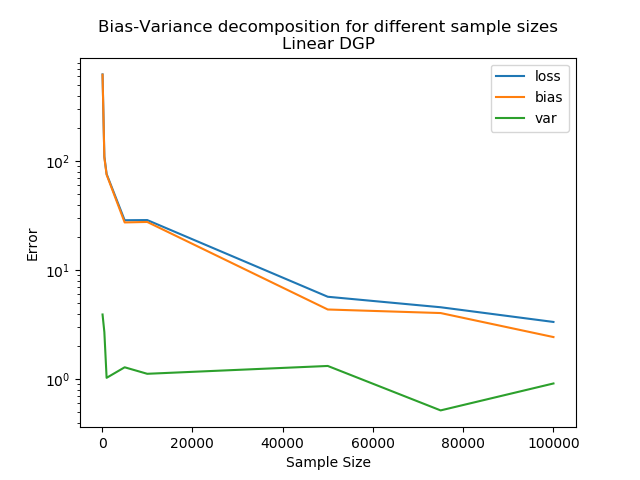
\includegraphics[width=120mm]{bias_var_linearDGP.png}}
	\caption{This figure demonstrates the decomposition of the expected generalization error in linear DGP. 
			The expected generalization error is denoted with loss. 
			As sample size increases both the expected generalization error and bias tend to decrease. 
			Although the variance does not follow a pattern, in theory, we expect low variance and 
			variance remains to be low for all sample sizes.}
	\label{fig:bias_var_linear}
\end{figure}

\begin{figure}[H]
	\centering
	\captionsetup{format=plain}
	\makebox{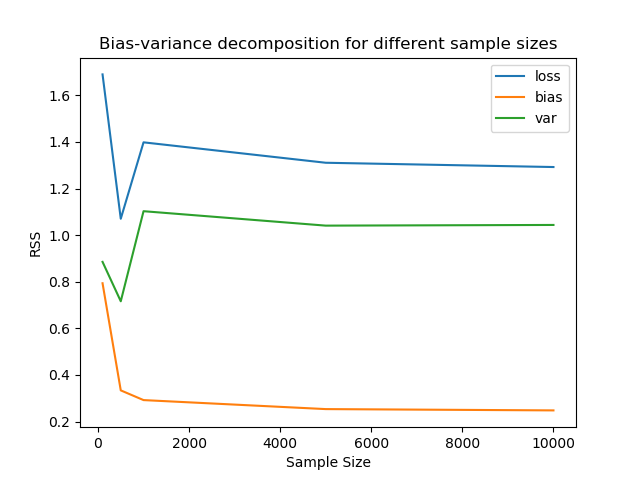
\includegraphics[width=120mm]{bias_var_nonlinearDGP.png}}
	\caption{This figure demonstrates the decomposition of the expected generalization error in nonlinear DGP. 
			The expected generalization error is denoted with loss. 
			The expected generalization error is driven primarily 
			by variance and bias remains to be low for all sample sizes. 
			As expected, Random Forest decreases the variance and bias remains to be low due to low biasness of Decision Tree estimates.}
	\label{fig:bias_var_nonlinear}
\end{figure}



